\appendix
\section{补充方法细节与提示词架构}
\label{sec:appendix_zh}

\subsection{观察与决策契约}
\label{app:prompt_zh}

观察包含账户、公共市场事实及私人记录。市场视图通过 \texttt{as\_of\_tick} 标记上一步的已提交行情，并提供当步政策状态和事件。私人记录包含画像、更新后的行为状态、所选消息和缓存。认知配置还提供从下一步开始可见的本人近期执行回执。

代码清单~\ref{lst:prompt_zh}示例为符合类型约束的观望响应。主体、观察及版本标识与本次请求对应。后端返回一个观望动作或一张有类型的委托，后者包含资产、方向、股数和整数报价档位。证据标识指向观察内可见事实。交易所在执行阶段校验价格和资源约束。

\noindent\begin{minipage}{\columnwidth}
\begin{lstlisting}[caption={观望动作响应示例。}, label={lst:prompt_zh}, basicstyle=\ttfamily\scriptsize, breaklines=true, frame=single, aboveskip=3pt, belowskip=3pt]
{
  "schema_version": 3,
  "decision_id": "decision-example",
  "actor_id": "agent-example",
  "observation_id": "observation-example",
  "batch_id": "batch-example",
  "observation_version": 1,
  "world_version": 1,
  "tick": 1,
  "policy_id": "kdd27_policy",
  "policy_version": "2",
  "economic_intents": [
    {"kind": "hold", "intent_id": "intent-example"}
  ],
  "evidence_ids": [],
  "belief_patch": {},
  "message_drafts": []
}
\end{lstlisting}
\end{minipage}

\section{基准配置与结果明细}
\label{app:benchmark_details_zh}

\paragraph{多日评价的参考配置。}
表~\ref{tab:params}与表~\ref{tab:behavior}记录长周期参考方案，其中 $N=10{,}000$、$T=20{,}000$、每个交易日 $T_{\rm day}=100$ 步，共 200 个交易日，含 50 日预热。日频协议计算有限样本校正的超额峰度、收益率和绝对收益率的 1--20 阶自相关，以及成交量与绝对收益率的相关性。表~\ref{tab:measured_design}单列本研究实际采用的基准配置。

% Market and Social Layer Default Configurations
\begin{table*}[t]
  \centering\small
  \caption{\tr{长周期参考设计的市场环境与社会传播参数。}{Market and social propagation parameters for the prospective multi-day design.}}
  \label{tab:params}
  \begin{tabularx}{\textwidth}{@{}l p{3.2cm} p{3.5cm} X@{}}
    \toprule
    \tr{模块}{Module} & \tr{参数}{Parameter} & \tr{设置}{Setting} & \tr{含义}{Meaning} \\
    \midrule
    \tr{执行}{Execution} & \tr{主体数、日内步数、仿真期限、预热期}{$N, T_{\mathrm{day}}$, horizon, burn-in} & \tr{$10^4$ 名主体，100 步/日\newline 200 日，预热 50 日}{$10^4$, $100$ steps, $200$ days, $50$ days} & \tr{种群规模、每个交易日的步数、总交易日数与预热日数}{Population, steps per day, horizon, and warm-up} \\
    \tr{账本}{Ledger} & $P_0, \mu_C, \sigma_C, Q_{\max}$ & $100, \log(10^5), 0.6, 2000$ & \tr{初始价格、对数正态现金分布与初始持仓上限}{Initial price, lognormal cash, and maximum initial shares} \\
    \tr{初始禀赋}{Endowments} & $\mu_K, \sigma_K, a_s, b_s$ & $100, 5, 2, 2$ & \tr{截断持仓成本分布与初始情绪 $s_{i,0}\in[-1,1]$ 的对称 Beta 抽样}{Truncated cost and symmetric Beta draws for $s_{i,0} \in [-1, 1]$} \\
    \tr{认知状态}{Cognition} & $q_0, \sigma_{q,0}, a_{i,0}, R^\bullet_{i,0}$ & $0.6, 0.1, 0.5, P_0$ & \tr{信心截断至 $[0,1]$，以及初始风险容忍度与价格参考点}{Confidence truncated to $[0,1]$, risk tolerance, and price anchors} \\
    \tr{网络拓扑}{Topology} & \tr{平均度 $k$、重连概率 $p$}{Mean degree $k$, rewiring $p$} & $6, 0.1$ & \tr{带聚类及短路径的 Watts--Strogatz 网络}{Watts--Strogatz network with clustering and shortcuts} \\
    \tr{边权}{Edge Weights} & $w_0, w_{\min}, w_{\max}, \omega$ & $1.0, 1.0, 2.0, 0.1$ & \tr{边权向 $2-|x_i^{\rm exp}-x_j^{\rm exp}|$ 调整}{Edge weights move toward $2-|x_i^{\rm exp}-x_j^{\rm exp}|$} \\
    \tr{消息筛选}{Information} & \tr{注意力容量 $A_i$、衰减 $\zeta_E$、权重 $\boldsymbol{\theta}$}{Capacity $A_i$, decay $\zeta_E$, weights $\boldsymbol{\theta}$} & $3, 0.05$,\newline$(0.35, 0.25, 0.15, 0.15, 0.10)$ & \tr{按情绪、主题、风险、影响力及曝光记录排序}{Attention-bounded filtering; ranking by emotion, topic, risk, influence, and exposure} \\
    \tr{传播}{Contagion} & \tr{基础感染率 $\beta$、恢复率 $\gamma$、免疫衰减 $\delta$}{Base infection $\beta$, recovery $\gamma$, waning $\delta$} & $0.30, 0.10, 0.05$ & \tr{社会联系上的离散时钟 SIRS 传播参数}{Discrete-time SIRS epidemiological parameters governing panic transmission across social edges} \\
    \tr{感染压力}{Pressure} & \tr{分量权重 $(\kappa_0,\kappa_1,\kappa_2)$}{Coupling weights $(\kappa_0, \kappa_1, \kappa_2)$} & $0.40, 0.40, 0.20$ & \tr{结合感染邻居和注意力筛选后信息的感染压力}{Multiscale infection pressure coupling infected-neighbor share and filtered exposure} \\
    \tr{回音室}{Echo Chamber} & \tr{持续时间 $\eta_d$、回音室 $\eta_e$、再易感 $\eta_\psi$}{Duration $\eta_d$, echo $\eta_e$, resusceptibility $\eta_\psi$} & $0.02, 0.50, 0.50$ & \tr{感染持续时间、曝光集中度与再次易感}{Duration, exposure concentration, and return to susceptibility} \\
    \tr{从众}{Herding} & \tr{悲观阈值 $s_*$、权重转移 $\eta_H$、信心更新 $\eta_q,\eta_{\mathrm{rec}}$}{Threshold $s_*$, shift $\eta_H$, learning $\eta_q, \eta_{\mathrm{rec}}$} & $0.20, 0.50, 0.05, 0.02$ & \tr{信心调节个人估值和同伴信号之间的权重转移}{Panic sentiment boundary; confidence-dependent cognitive weight reallocation to peer consensus} \\
    \tr{市场制度}{Microstructure} & \tr{佣金 $c$、印花税 $\tau^{\mathrm{tax}}$、价带 $L$、价格档位 $\Delta_p$}{Fee $c$, stamp tax $\tau^{\mathrm{tax}}$, band $L$, tick $\Delta_p$} & $0.025\%, 0.05\%, 10\%, 0.01$ & \tr{双边佣金、卖方税、日价格限制与最小报价单位}{Bilateral commission, seller-side transaction tax, daily price fluctuation limit, and price tick} \\
    \tr{订单规则}{Order Rules} & \tr{活跃率 $p_{\mathrm{act}}$、有效期、$T+1$ 限制}{Activity rate $p_{\mathrm{act}}$, lifespan, T+1 limit} & \tr{$p_{\mathrm{act}}=0.05$，有效期 1 步\newline $T+1$ 可配置}{$0.05$, $1$ step, configurable} & \tr{伯努利活跃概率、未成交订单的撤单期限与当日回转限制}{Bernoulli activity probability, unexecuted order cancellation horizon, and day-trade turnover restriction} \\
    \bottomrule
  \end{tabularx}
\end{table*}

% Behavioral and Cognitive Core Parameters
\begin{table*}[t]
  \centering\small
  \caption{\tr{参考设计中的估值、委托与认知参数。}{Valuation, order, and cognition parameters in the reference design.}}
  \label{tab:behavior}
  \begin{tabularx}{\textwidth}{@{}l p{3.2cm} p{3.5cm} X@{}}
    \toprule
    \tr{模块}{Module} & \tr{参数}{Parameter} & \tr{设置}{Setting} & \tr{含义}{Meaning} \\
    \midrule
    \tr{前景理论}{Prospect Theory} & \tr{损失厌恶 $\lambda_i$、幂指数 $\alpha$、缩放系数 $\kappa_v$}{Loss aversion $\lambda_i$, power $\alpha$, scale $\kappa_v$} & \mbox{2.25, 0.88, 10} & \tr{参考依赖价值函数。$\alpha$ 与 $\lambda$ 取自文献，$\kappa_v$ 为模型设定}{Reference-dependent value; $\alpha$ and $\lambda$ follow literature values, $\kappa_v$ is a model choice} \\
    \tr{参考点更新}{Reference Dynamics} & \tr{记忆速率 $(\kappa_p, \kappa_h, \kappa_n, \kappa_e)$}{Memory rates $(\kappa_p, \kappa_h, \kappa_n, \kappa_e)$} & $(0.03, 0.10, 0.16, 0.18)$ & \tr{持仓成本、滚动高点、同伴与政策参考点的更新速率}{Adaptive update rates for purchase cost, local rolling peak, peer consensus, and policy anchor} \\
    \tr{参考点权重}{Reference Weights} & \tr{参考点权重 $(\omega_p, \omega_h, \omega_n, \omega_e)$}{Anchor weights $(\omega_p, \omega_h, \omega_n, \omega_e)$} & $(0.34, 0.26, 0.20, 0.20)$ & \tr{多参考点心理账户，滚动窗口 $H_h=100$ 步，参考点目标幅度 $\xi_n=\xi_e=0.05$}{Multi-reference mental accounting; $H_h = 100$ rolling steps, reference-target amplitudes $\xi_n = \xi_e = 0.05$} \\
    \tr{损失压力}{Loss Pressure} & \tr{敏感度 $\chi$、上下界 $[\ell_{\min},\ell_{\max}]$、损失缩放 $\nu$}{Coupling $\chi$, bounds $[\ell_{\min}, \ell_{\max}]$, loss-penalty scale $\nu$} & \tr{$\chi=0.50$，$[1.0,5.0]$\newline $\nu=4.0$}{$0.50, [1.0, 5.0], 4.0$} & \tr{由持仓成本及近期高点驱动的损失压力}{Reference-loss pressure based on cost and high-price anchors} \\
    \tr{风险容忍度}{Risk Preference} & \tr{动态权重 $\boldsymbol{\omega}_a$}{Dynamic weights $\boldsymbol{\omega}_a$} & $(0.35, 0.45, 0.10, 0.10, 0.15)$ & \tr{信心、上一期风险容忍度、情绪、估值方向、损失惩罚权重}{Weights on confidence, previous risk, emotion, direction, and loss penalty} \\
    \tr{订单生成}{Order Generation} & \tr{缩放系数 $\kappa_a$、阈值 $\delta_a$、投入范围 $[f_{\min},f_{\max}]$}{Scale $\kappa_a$, threshold $\delta_a$, limits $[f_{\min}, f_{\max}]$} & $5.0, 0.25, [0.01, 0.10]$ & \tr{交易意图至委托的映射及资源投入比例}{Intent-to-order mapping; fraction of available liquidity deployed per active trading step} \\
    \tr{交易意图}{Intention} & \tr{权重 $(\omega_\tau^d,\omega_\tau^s,\omega_\tau^a)$}{Weights $(\omega_\tau^d,\omega_\tau^s,\omega_\tau^a)$} & $(0.45,0.40,0.15)$ & \tr{估值方向、情绪与风险容忍度权重}{Valuation direction, sentiment, and risk tolerance} \\
    \tr{报价}{Quote Pricing} & \tr{扰动 $\sigma_p$、价格档位 $\Delta_p$}{Perturbation $\sigma_p$, tick size $\Delta_p$} & $0.002, 0.01$ & \tr{以上一提交价格为中心作均值校正的对数正态扰动}{Mean-corrected log-normal quote dispersion around the previous committed price} \\
    \tr{情绪权重}{Emotion Weights} & \tr{技术型、新闻型、从众型}{Technical / News / Herding styles} & \shortstack[l]{$(.6,.1,.1,.2)$\\$(.35,.35,.2,.1)$\\$(.25,.15,.5,.1)$} & \tr{不同风格的惯性、感染、同伴与上一期收益权重}{Weights on inertia, infection, peers, and prior return by cognitive style} \\
    \tr{双速混合调度}{Dual-Speed Hybrid} & \tr{慢组人数 $k$、周期 $T_{\mathrm{slow}}$、缓存寿命 $A_{\max}$}{Count $k$, period $T_{\mathrm{slow}}$, cache TTL $A_{\max}$} & \tr{$10$、10 步、10 步}{$10, 10\text{ steps}, 10\text{ steps}$} & \tr{认知参考配置的慢组人数、请求周期与缓存有效期}{Slow group size, request period, and cache lifetime in the cognition profile} \\
    \tr{主体记忆}{Agent Memory} & \tr{衰减尺度 $S_m$、最大条目 $M_{\max}$}{Decay factor $S_m$, max items $M_{\max}$} & \tr{$100$ 步、8}{$100\text{ steps}, 8$} & \tr{主体自己的近期执行回执与记忆衰减尺度}{Own execution receipts and their decay scale in the cognition profile} \\
    \bottomrule
  \end{tabularx}
\end{table*}


\paragraph{基准结果明细。}
表~\ref{tab:invariants}逐条报告账本核验。表~\ref{tab:rq1_results}汇总日内轨迹，表~\ref{tab:rq2_results}报告全部共同父世界分支的结果。表~\ref{tab:pilot}和表~\ref{tab:rq3_results}分别记录决策计数与计算开销。

\begin{table*}[t]
  \centering\small
  \caption{\tr{各匹配种子的账本守恒与终态恢复。同平台只读恢复结果与各归档的终态哈希一致。}{Ledger conservation and terminal restoration for each matched seed. Read-only restorations on the same platform reproduce the archived terminal state hashes.}}
  \label{tab:invariants}
  \begin{tabularx}{\textwidth}{@{}l X r r r r c@{}}
    \toprule
    \tr{种子}{Seed} & \tr{交易策略}{Trading policy} & \tr{提交步数}{Commits} & \tr{现金残差}{Cash residual} & \tr{股份残差}{Share residual} & \tr{税费残差}{Fee residual} & \tr{终态哈希}{Terminal hash}\\
    \midrule
    932201 & \tr{完整模型}{Full model} & 100 & 0 & 0 & 0 & \tr{匹配}{Match} \\
    932201 & \tr{零智能}{Zero intelligence} & 100 & 0 & 0 & 0 & \tr{匹配}{Match} \\
    932201 & \tr{同质线性价值}{Linear value} & 100 & 0 & 0 & 0 & \tr{匹配}{Match} \\
    932202 & \tr{完整模型}{Full model} & 100 & 0 & 0 & 0 & \tr{匹配}{Match} \\
    932202 & \tr{零智能}{Zero intelligence} & 100 & 0 & 0 & 0 & \tr{匹配}{Match} \\
    932202 & \tr{同质线性价值}{Linear value} & 100 & 0 & 0 & 0 & \tr{匹配}{Match} \\
    932203 & \tr{完整模型}{Full model} & 100 & 0 & 0 & 0 & \tr{匹配}{Match} \\
    932203 & \tr{零智能}{Zero intelligence} & 100 & 0 & 0 & 0 & \tr{匹配}{Match} \\
    932203 & \tr{同质线性价值}{Linear value} & 100 & 0 & 0 & 0 & \tr{匹配}{Match} \\
    \bottomrule
  \end{tabularx}
\end{table*}

% Generated from packaged archive data by scripts/render_real_figures.py
\begin{table*}[t]
\centering\small
\caption{\tr{RQ1 日内市场活动与盘口流动性。每种模型包含三个匹配种子的轨迹（$N=100,T=100$）。各指标报告均值及 [最小值, 最大值]。}{RQ1 Intraday Market Activity and Quoted Liquidity. Each model has three matched-seed trajectories ($N=100,T=100$). Entries report mean [minimum, maximum].}}
\label{tab:rq1_results}
\begin{tabularx}{\textwidth}{@{}l r X X X X@{}}
\toprule
Baseline & Worlds & No trade (\%) & One-sided book (\%) & Two-sided quotes (\%) & Trades \\
\midrule
Civitas full model & 3 & 69.67 [66, 76] & 71.67 [69, 76] & 18.33 [18, 19] & 43.67 [34, 57] \\
Zero intelligence & 3 & 70.33 [66, 78] & 70.67 [68, 73] & 16.00 [11, 20] & 42.67 [34, 50] \\
Homogeneous linear value & 3 & 70.67 [61, 78] & 68.33 [64, 73] & 20.33 [13, 24] & 44.67 [36, 55] \\
\bottomrule
\end{tabularx}
\end{table*}

% Generated from packaged archive data by scripts/render_real_figures.py
\begin{table*}[t]
\centering\small
\caption{\tr{RQ2 共同父世界的十一条干预分支（$N=20$，27 步事件窗口）。感染峰值取事件窗口内逐步感染比例的最大值。星号标记窗口终点的右删失。}{RQ2 Outcomes for Eleven Intervention Branches from a Shared Parent World ($N=20$, 27 event steps). Peak infection is the maximum stepwise infection share within the event window. An asterisk marks right censoring at the window endpoint.}}
\label{tab:rq2_results}
\begin{tabularx}{\textwidth}{@{}l c c c c c X@{}}
\toprule
Intervention & MDD (\%) & Peak infection (\%) & Relative turnover & Confirmation (steps) & Censored & Tradable steps \\
\midrule
Full control & 0.4754 & 45 & 1.0000 & 20 & No & 27/27 \\
Secondary spread off & 0.1453 & 5 & 0.8076 & 20 & No & 27/27 \\
No herding & 0.4754 & 45 & 0.9797 & 20 & No & 27/27 \\
Both off & 0.1453 & 5 & 0.8076 & 20 & No & 27/27 \\
Loss feedback off & 0.4759 & 45 & 0.8962 & 20 & No & 27/27 \\
$\lambda=1$ & 0.4759 & 45 & 0.8962 & 20 & No & 27/27 \\
Valuation sign reversed & 1.6372 & 45 & 1.7873 & 27$^{*}$ & Yes & 27/27 \\
Halt (25 steps) & 0.0000 & 45 & 0.1772 & 20 & No & 2/27 \\
Seller tax 0.15\% & 0.4754 & 45 & 1.0000 & 20 & No & 27/27 \\
T+1 lock & 0.4754 & 45 & 1.0000 & 20 & No & 27/27 \\
Price band 5\% & 0.4754 & 45 & 1.0000 & 20 & No & 27/27 \\
\bottomrule
\end{tabularx}
\end{table*}

\begin{table*}[t]
  \centering\small
  \caption{\tr{九类画像及三类配对对比的固定观察响应。各后端均在相同的 54 个请求单元上评价。变化计数以每类九对为分母。}{Fixed-observation responses across nine archetypes and three paired contrasts. All backends use the same 54 cells. Signature changes are counted out of nine pairs per contrast.}}
  \label{tab:pilot}
  \begin{tabularx}{\textwidth}{@{}X rrr c ccc@{}}
    \toprule
    \tr{决策后端}{Backend} & HOLD & BUY & SELL & \tr{资源可行}{Resource feasible} &
    \tr{价格签名变化}{Price changes} & \tr{锁定签名变化}{Lock changes} & \tr{现金签名变化}{Cash changes} \\
    \midrule
    \tr{数值规则}{Numerical rules} & 9 & 45 & 0 & 54/54 & 9/9 & 0/9 & 9/9 \\
    \tr{画像启发式}{Persona heuristics} & 27 & 9 & 18 & 54/54 & 7/9 & 1/9 & 8/9 \\
    \tr{真实 LLM}{Live LLM} & 54 & 0 & 0 & 54/54 & 0/9 & 0/9 & \mbox{0/9} \\
    \bottomrule
  \end{tabularx}
\end{table*}

% Generated from packaged archive data by scripts/render_real_figures.py
\begin{table*}[t]
\centering\small
\caption{\tr{模型请求与规则世界的实测计算记录。$^{a}$ 快照批次壁钟时间。规则世界的运行剖面包括终态检查点。$^{b}$ ASUS 内存为采样峰值，最终运行剖面缺失。}{Measured Compute for Model Requests and Rule Worlds. $^{a}$~Snapshot batch wall time. Rule-world profiles include terminal checkpoints. $^{b}$~ASUS memory is the sampled peak. Its final profile is unavailable.}}
\label{tab:rq3_results}
\begin{tabularx}{\textwidth}{@{}l r c c c X@{}}
\toprule
Measured workload & Live calls & Input / output tokens & Time (s) & Memory (GiB) & Completion status \\
\midrule
Live snapshot batch & 54 & 119,637 / 9,306 & 69.597$^{a}$ & --- & 54/54 responses; all HOLD \\
Mac: $N=100,T=100$ & 0 & 0 / 0 & 1862.397 & 1.239 & Runner/controller complete \\
Mac: $N=100,T=200$ & 0 & 0 / 0 & 7619.767 & 2.486 & Runner/controller complete \\
ASUS: $N=1000,T=12$ & 0 & 0 / 0 & Missing & 1.692$^{b}$ & Runner saved 12 steps; controller stopped \\
\bottomrule
\end{tabularx}
\end{table*}


\section{调度与校验器诊断}
\label{app:timing_zh}

调度核对使用 $N=100$、$T=4{,}000$ 的认知参考配置及 20 个固定种子的活跃掩码。在仿真步 1,200，所有主体的市场视图均含有公告。按计划发出包含文本的请求，需要主体在该步活跃并符合模型请求资格。图~\ref{fig:schedule_exposure_zh}右图给出逐种子计数。

两种严格校验器处理同一个 $N=100$、$T=12$ 的规则世界。图~\ref{fig:timing_supp_zh}给出三组配对计时。

\begin{figure*}[t]
 \centering
 \begin{subfigure}{0.96\textwidth}
  \centering
  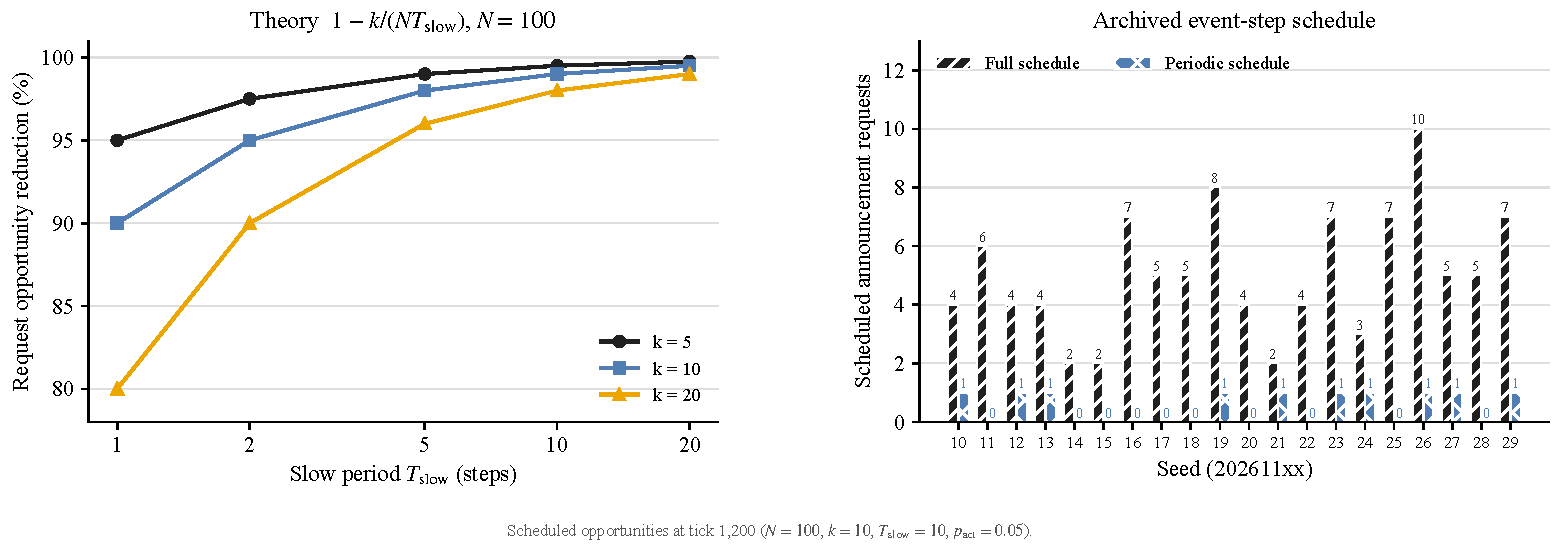
\includegraphics[width=\textwidth]{figures/schedule_exposure.pdf}
  \caption{期望请求缩减与公告请求资格。}
  \label{fig:schedule_exposure_zh}
 \end{subfigure}
 \par\medskip
 \begin{subfigure}{0.55\textwidth}
  \centering
  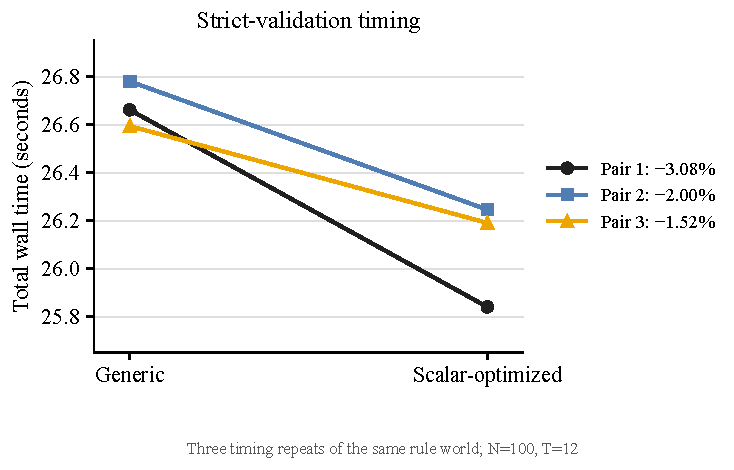
\includegraphics[width=\textwidth]{figures/engineering_timing.pdf}
  \caption{两种严格校验器的配对壁钟耗时。}
  \label{fig:timing_supp_zh}
 \end{subfigure}
 \caption{调度与校验器诊断。（a）左图设 $N=100$、期限为周期整数倍，改变周期 $T_{\mathrm{slow}}$ 与慢组人数 $k$。右图记录公告发布时具备请求资格的活跃主体数。（b）各条连线连接同一规则世界下通用与标量优化校验器的配对计时。}
 \Description{调度的期望请求缩减率、20 个种子的公告请求资格计数和严格校验配对计时。}
\end{figure*}
